\documentclass[10pt,twocolumn]{article}

% --- Mini research-paper style (self-contained; compiles on Overleaf or any
% --- TeX Live with no extra .sty files). Mimics a typical ML-conference look.
\usepackage[a4paper,margin=0.75in]{geometry}
\usepackage[T1]{fontenc}
\usepackage{times}
\usepackage{graphicx}
\usepackage{amsmath,amssymb}
\usepackage{booktabs}
\usepackage{caption}
\usepackage{authblk}
\usepackage[hidelinks]{hyperref}
\usepackage{xcolor}

\captionsetup{font=small,labelfont=bf}
\setlength{\parskip}{0.2em}
\newcommand{\eps}{\varepsilon}
\newcommand{\obs}{\texttt{obs}}
\newcommand{\qv}{\texttt{q\_values}}
\newcommand{\hid}{\texttt{hidden}}

\title{\vspace{-2em}\textbf{Correlated Exploration for Cooperative MARL\\via a Gaussian Copula}}
\author[]{Micha\l{} S\l owakiewicz \and Jakub Wo\'zniak}
\affil[]{Project 9 --- Reinforcement Learning}
\date{}

\begin{document}
\maketitle

\begin{abstract}
\small
In cooperative multi-agent RL (MARL), agents must often \emph{coordinate} their
actions to receive any reward. Standard $\eps$-greedy explores each agent
independently, so the chance of stumbling on a coordinated joint action decays
exponentially in the number of agents. We replace independent $\eps$-greedy with
\textbf{correlated $\eps$-greedy}: the random action that exploring agents take
is coupled through a Gaussian copula whose correlation matrix is the cosine
similarity of per-agent features, so similar agents tend to pick the same action.
On a coordination-bottlenecked toy task (\emph{Hallway}) this yields a
\textbf{+64--94\%} relative early-learning gain; on sparse \emph{Level-Based
Foraging} it finds \textbf{2.6--2.9$\times$} more coordinated successes; and on a
GPU-scale StarCraft-like task (SMAX \texttt{2s3z}, JAX) it makes QMIX training
markedly more reliable (mean final win $0.81{\to}0.91$ with $\sim$3$\times$ lower
seed variance; suggestive but not significant at $n{=}5$). The observation is the
most reliable similarity source, coupling situationally-similar agents with no
role information supplied.
\end{abstract}

\section{Introduction}
We study the decentralised partially-observable MDP (Dec-POMDP) under centralised
training, decentralised execution (CTDE): each agent $i$ observes $o_i$, picks
$a_i$, and the team receives a single shared reward $r$.

\paragraph{The coordination problem.} Consider a task that rewards the team only
when all $n$ agents simultaneously take a specific matching action. Under
independent $\eps$-greedy, the probability that all $n$ explore the matching
joint action in one step is $\propto \eps^{n}$ --- exponentially small. If agents
instead explored in a \emph{correlated} way, tending to take similar actions
together, they would sample coordinated joint actions far more often.

\paragraph{Hypothesis.} \emph{Replacing independent $\eps$-greedy with correlated
exploration, where the correlation reflects how similar two agents currently are,
accelerates learning on coordination-bottlenecked tasks.}

\section{Method}
We keep the $\eps$-greedy template --- with probability $\eps$ an agent acts
randomly, else greedily --- but \emph{correlate which random action exploring
agents take}. \emph{Who} explores stays an independent Bernoulli (same
exploration budget as the baseline); only the random action is coupled.

\paragraph{Gaussian copula.} A copula imposes a desired correlation on uniform
variables while keeping each marginal uniform. Given a correlation matrix $R$
(PSD, unit diagonal): (i)~factorise $R=LL^\top$; (ii)~sample
$z\sim\mathcal{N}(0,I)$ and set $y=Lz\sim\mathcal{N}(0,R)$; (iii)~map
$u_i=\Phi(y_i)$, giving uniform marginals \emph{correlated} according to $R$. An
exploring agent then takes the action $\lfloor u_i\,|A_i|\rfloor$ among its
$|A_i|$ available actions. Because the $u_i$ are correlated, agents with high
$R_{ij}$ pick the \emph{same} action --- a coordinated joint action (both stepping
on switches, or focus-firing the same enemy). Independent $\eps$-greedy is the
special case $R=I$.

\paragraph{Correlation from cosine similarity.} Let $f_i$ be a feature vector for
agent $i$ and $\hat f_i = f_i/\lVert f_i\rVert$. Then
\begin{equation}
R_{ij}=\hat f_i^\top \hat f_j=\frac{f_i^\top f_j}{\lVert f_i\rVert\,\lVert f_j\rVert}=\cos\theta_{ij},
\quad R=\hat F\hat F^\top+\lambda I,
\end{equation}
where $\hat F$ stacks the normalised features. $R$ is a Gram matrix, hence
positive semi-definite ($x^\top R x=\lVert\hat F^\top x\rVert^2\ge 0$) with unit
diagonal --- a valid correlation matrix; the jitter $\lambda=10^{-3}$ keeps the
Cholesky well-conditioned. We compare three similarity sources $f_i$: the
(augmented) observation \obs, the Q-value vector \qv, and the Q-network backbone
activation \hid. The design is role-agnostic: nothing tells the method which
agents share a role; similar agents simply get correlated.

\section{Experimental Setup}
\textbf{Environments.}
\emph{Hallway}~\cite{maven}: two agents on separate corridors (lengths 3, 4),
each seeing only its own position; the team is rewarded only when both reach
position~0 in the same step.
\emph{Level-Based Foraging}~\cite{lbf} (\texttt{Foraging-5x5-2p-1f-coop}): two
agents must load one food item \emph{together}; sparse reward.
\emph{SMAX \texttt{2s3z}}~\cite{jaxmarl}: a JAX StarCraft-like battle, 2 stalkers
$+$ 3 zealots vs.\ a mirrored enemy team --- a 5-agent, two-role task.

\textbf{Algorithms.} Two value-decomposition backbones with parameter sharing
(one shared Q-net; agents disambiguated by a one-hot id): VDN~\cite{vdn}
($Q_{\text{tot}}=\sum_i Q_i$) and QMIX~\cite{qmix} (monotonic mixer with a
hypernetwork over the global state). DQN-style training, 5 seeds per
configuration. On LBF we oversample the rare successful transitions
(balanced replay).

\section{Results: Toy Benchmarks}

\begin{figure}[t]
\centering
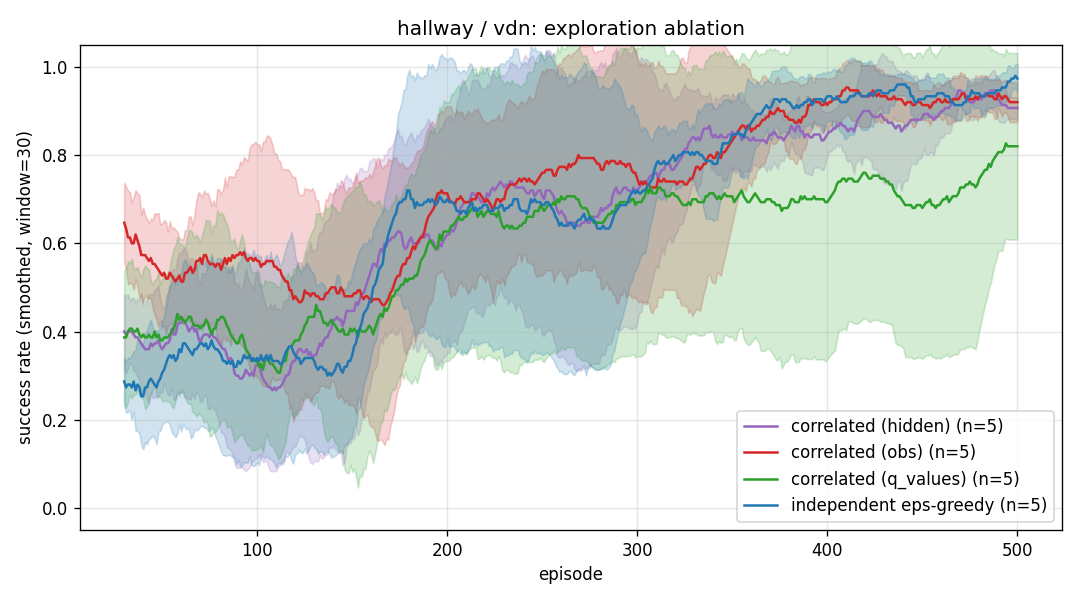
\includegraphics[width=\linewidth]{plot_hallway_vdn.png}
\caption{\emph{Hallway} (VDN). Correlated-\obs{} learns markedly faster early;
all variants converge, so the gain is a speed-up.}
\label{fig:hallway}
\end{figure}

\paragraph{Hallway: faster early learning.} Correlated exploration with the \obs{}
source learns markedly faster in the early phase, when exploration matters most
(Fig.~\ref{fig:hallway}, Table~\ref{tab:hallway}). All variants eventually reach
a high success rate, so the benefit is a \textbf{speed-up}, exactly as the
hypothesis predicts for a coordination-bottlenecked task.

\begin{table}[t]
\centering\small
\caption{Hallway success rate at episodes 50--100.}
\label{tab:hallway}
\begin{tabular}{lccc}
\toprule
Backbone & Independent & Correlated-\obs & Relative \\
\midrule
VDN  & 0.348 & \textbf{0.572} & +64\% \\
QMIX & 0.276 & \textbf{0.536} & +94\% \\
\bottomrule
\end{tabular}
\end{table}

\begin{figure}[t]
\centering

\includegraphics[width=\linewidth]{plot_lbf_vdn.png}
\caption{\emph{LBF} (VDN). All methods collapse (catastrophic forgetting), but
correlated reaches a 2.6--2.9$\times$ higher \emph{peak}.}
\label{fig:lbf}
\end{figure}

\paragraph{LBF: the mechanism works even where learning fails.} LBF is dominated
by catastrophic forgetting --- every method peaks early then collapses toward
zero (Fig.~\ref{fig:lbf}). The \emph{peak} success rate, however, cleanly
separates the methods: independent peaks at 0.07--0.09, while the best correlated
variant peaks at 0.20--0.24 --- \textbf{2.6--2.9$\times$ higher}. The exploration
mechanism finds the coordinated successes independent exploration misses; failing
to \emph{retain} them is a separate problem of value learning under extreme
sparsity.

\paragraph{Which similarity source?} \obs{} is the most reliable: it gives the
largest, most consistent early gain and the highest LBF peak. \qv{} and \hid{}
are inconsistent --- early in training the network is random, so its Q-values and
activations carry little reliable signal, whereas the observation is informative
from step one.

\section{Results: SMAX \texttt{2s3z} (JAX, GPU)}
We reimplemented the method in pure JAX (Flax/Optax), vectorising 128 parallel
environments with \texttt{jax.vmap} ($\sim$6900 env-steps/s on one RTX 2080 Ti).

\paragraph{Stabilising a from-scratch learner.} Our first runs did not learn:
the TD loss \emph{diverged} to $10^4$--$10^6$ (Q-value explosion, not
under-training). Four standard fixes resolved it --- Double DQN~\cite{ddqn}
targets, Polyak soft target updates ($\tau{=}0.005$), $\text{lr}=10^{-4}$, and a
\texttt{LayerNorm} on the QMIX mixer's unnormalised global-state input (values up
to $\sim$24 otherwise blew up the $\mathrm{abs}()$-weighted hypernetwork). The
best configurations then reach a 95--100\% win rate.

\begin{figure}[t]
\centering
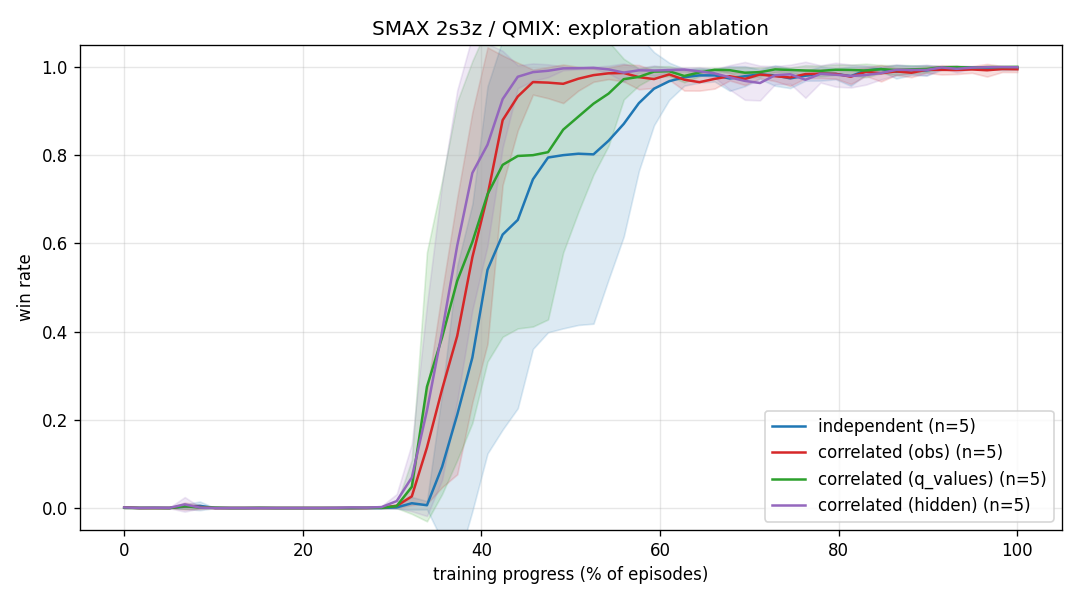
\includegraphics[width=\linewidth]{plot_smax_qmix.png}
\caption{SMAX \texttt{2s3z} (QMIX). Correlated variants reach a higher final win
rate than independent (0.91 vs.\ 0.81) and get there sooner.}
\label{fig:smax}
\end{figure}

\paragraph{Correlated exploration helps most on the harder mixer.}
Under VDN (simple additive mixer) every variant converges to $\sim$0.95;
correlated only reaches the 50\%-win milestone $\sim$6\% sooner. Under QMIX
(harder monotonic mixer) the effect is larger but must be read carefully
(Table~\ref{tab:smax}, Fig.~\ref{fig:smax}): independent has a much higher mean
\emph{and} a much larger seed variance ($0.81{\pm}0.19$; one seed collapses to
$0.48$), while all correlated variants are higher and far more reliable
($0.90$--$0.91$, std $\le 0.12$). A bootstrap over the 5 seeds gives a mean gap of
$+0.10$ for the best correlated variant with 95\% CI $[-0.03, 0.28]$ and
$P(\text{correlated}>\text{independent})\approx 0.91$ --- \emph{suggestive but not
significant at $n{=}5$}. The robust, reproducible effect is therefore the
\textbf{reduced variance / improved reliability} of correlated exploration (it
avoids the failed runs that independent suffers) plus the consistent early
speed-up; a firm claim on the mean final-win gain would need more seeds.

\begin{table}[t]
\centering\small
\caption{SMAX \texttt{2s3z}: final win rate (mean\,$\pm$\,std over 5 seeds).}
\label{tab:smax}
\setlength{\tabcolsep}{3pt}
\begin{tabular}{lcccc}
\toprule
& Indep. & corr-\obs & corr-\qv & corr-\hid \\
\midrule
VDN  & $0.95{\pm}.02$ & $0.95{\pm}.01$ & $0.94{\pm}.01$ & $0.95{\pm}.01$ \\
QMIX & $0.81{\pm}.19$ & $0.91{\pm}.06$ & $0.90{\pm}.12$ & $0.91{\pm}.07$ \\
\bottomrule
\end{tabular}
\end{table}

\begin{figure}[t]
\centering
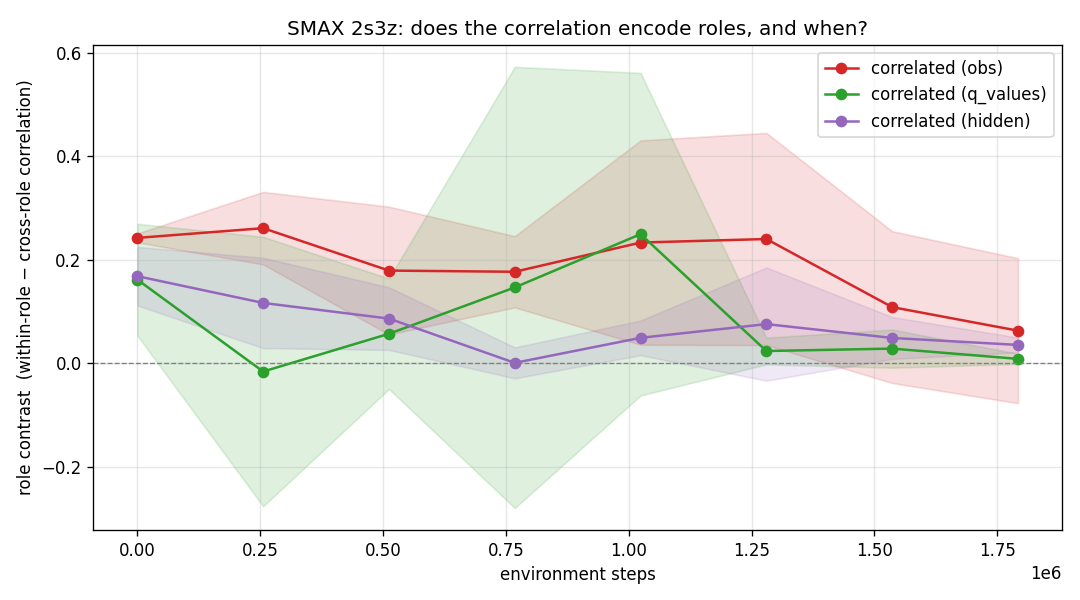
\includegraphics[width=\linewidth]{plot_smax_corr_evolution.png}
\caption{Role contrast (within-role $-$ cross-role correlation) over training.
\obs{} stays positive through the exploration-heavy phase; \qv{} is noisy and
\hid{} weak.}
\label{fig:contrast}
\end{figure}

\paragraph{When does the correlation encode roles?} The copula recomputes $R$
live, and exploration peaks early (high $\eps$), so \emph{when} $R$ carries role
structure matters. We summarise each snapshot by a role-contrast score
(within-role minus cross-role correlation; Fig.~\ref{fig:contrast}). \obs{} keeps
a clearly positive contrast through the exploration-heavy phase --- the
observation always encodes unit type, independent of the (initially random)
network. \qv{} is noisy and \hid{} weak. By convergence \qv{} is essentially
uniform ($\sim$0.99): a converged policy has large, all-positive Q-vectors, and
cosine between two large positive vectors is dominated by their shared offset
(mean-centring drops it to $\sim$0.85), so \qv{} cannot discriminate agents.
The \obs{} coupling is largely aligned with unit type --- the two stalkers are
consistently the most-correlated pair ($\sim$0.9) --- but reflects
\emph{situational} similarity (positions, visible enemies), not a clean role
partition: which zealot couples with the stalkers varies by seed. Coupling
situationally-similar agents is arguably the right behaviour.

\section{Discussion and Conclusion}
Correlated exploration helps where (a) coordination is the bottleneck and (b)
learning is stable enough to exploit discovered successes (Hallway, SMAX-QMIX).
Where learning itself is unstable (LBF), it still finds more successes but the
gain is not retained. \obs{} is the safe default similarity source.

\paragraph{Limitations.} (i)~The \emph{Hallway} observation is a single
non-negative scalar, so its cosine matrix is $\approx$ all-ones regardless of
state; there correlated-\obs{} reduces to ``explore the same action.'' That
validates \emph{that} correlated exploration helps, but not the discriminative
value of the cosine similarity --- which is genuinely exercised only by the
higher-dimensional LBF and SMAX observations. (ii)~The SMAX final-win
improvement is suggestive but not significant at $n{=}5$ (Sec.~5); the robust
claim is the reduced variance and faster learning. (iii)~We correlate actions
only \emph{within a single step}, unlike trajectory-level committed exploration
(e.g.\ MAVEN); per-step coupling already raises the rate of coordinated joint
actions, but temporally-extended coupling is a natural extension. (iv)~$R$ is
recomputed greedily each step rather than annealed; only 2 agents in the toy
tasks.

Overall, coupling agents' exploratory \emph{actions} through a Gaussian copula
parameterised by cosine similarity is a simple, drop-in change that measurably
accelerates cooperative MARL on coordination-bottlenecked tasks and improves
exploration quality even where value learning fails --- scaling from toy grids to
a GPU-scale StarCraft-like task.

\section*{Use of AI Tools}
\small
During the development of this project, \textbf{Claude Code} (Anthropic Claude
Opus) was used as a programming assistant: implementing substantial parts of the
PyTorch toy-environment stack and the JAX/JaxMARL SMAX pipeline, assisting with
cluster debugging (e.g., resolving CUDA/cuDNN compatibility and multi-process GPU
OOM issues), generating figures, and helping draft this report.
\emph{Worked well:} the tool was effective for rapid prototyping and for
diagnosing specific implementation bottlenecks --- notably the SMAX Q-divergence
and the $\sim$50$\times$ \texttt{vmap} speed-up.
\emph{Did not:} the assistant occasionally produced conceptually flawed logic.
Most notably, its initial SMAX exploration strategy correlated \emph{whether}
each agent explored rather than \emph{which action} it took --- a critical
conceptual bug that surfaced only under manual code review. Ultimately, while the
tool accelerates implementation, human oversight and conceptual verification
remained necessary throughout.

\begin{thebibliography}{9}
\small
\bibitem{vdn} P.~Sunehag et al. Value-Decomposition Networks for Cooperative
Multi-Agent Learning. \emph{AAMAS}, 2018.
\bibitem{qmix} T.~Rashid et al. QMIX: Monotonic Value Function Factorisation for
Deep Multi-Agent RL. \emph{ICML}, 2018.
\bibitem{maven} A.~Mahajan et al. MAVEN: Multi-Agent Variational Exploration.
\emph{NeurIPS}, 2019.
\bibitem{jaxmarl} A.~Rutherford et al. JaxMARL: Multi-Agent RL Environments and
Algorithms in JAX. 2023.
\bibitem{ddqn} H.~van Hasselt, A.~Guez, D.~Silver. Deep RL with Double
Q-learning. \emph{AAAI}, 2016.
\bibitem{lbf} G.~Papoudakis et al. Benchmarking Multi-Agent Deep RL Algorithms in
Cooperative Tasks. \emph{NeurIPS Datasets \& Benchmarks}, 2021.
\end{thebibliography}

\end{document}
